% Options for packages loaded elsewhere
\PassOptionsToPackage{unicode}{hyperref}
\PassOptionsToPackage{hyphens}{url}
%
\documentclass[
  english,
  man]{apa6}
\usepackage{lmodern}
\usepackage{amssymb,amsmath}
\usepackage{ifxetex,ifluatex}
\ifnum 0\ifxetex 1\fi\ifluatex 1\fi=0 % if pdftex
  \usepackage[T1]{fontenc}
  \usepackage[utf8]{inputenc}
  \usepackage{textcomp} % provide euro and other symbols
\else % if luatex or xetex
  \usepackage{unicode-math}
  \defaultfontfeatures{Scale=MatchLowercase}
  \defaultfontfeatures[\rmfamily]{Ligatures=TeX,Scale=1}
\fi
% Use upquote if available, for straight quotes in verbatim environments
\IfFileExists{upquote.sty}{\usepackage{upquote}}{}
\IfFileExists{microtype.sty}{% use microtype if available
  \usepackage[]{microtype}
  \UseMicrotypeSet[protrusion]{basicmath} % disable protrusion for tt fonts
}{}
\makeatletter
\@ifundefined{KOMAClassName}{% if non-KOMA class
  \IfFileExists{parskip.sty}{%
    \usepackage{parskip}
  }{% else
    \setlength{\parindent}{0pt}
    \setlength{\parskip}{6pt plus 2pt minus 1pt}}
}{% if KOMA class
  \KOMAoptions{parskip=half}}
\makeatother
\usepackage{xcolor}
\IfFileExists{xurl.sty}{\usepackage{xurl}}{} % add URL line breaks if available
\IfFileExists{bookmark.sty}{\usepackage{bookmark}}{\usepackage{hyperref}}
\hypersetup{
  pdftitle={Sexism and Division of Labor on Feelings of Teamliness Within Household Dyads},
  pdfauthor={Naomi Liftman1 \& Cara Krupnikoff-Salkin1},
  pdflang={en-EN},
  pdfkeywords={keywords},
  hidelinks,
  pdfcreator={LaTeX via pandoc}}
\urlstyle{same} % disable monospaced font for URLs
\usepackage{graphicx,grffile}
\makeatletter
\def\maxwidth{\ifdim\Gin@nat@width>\linewidth\linewidth\else\Gin@nat@width\fi}
\def\maxheight{\ifdim\Gin@nat@height>\textheight\textheight\else\Gin@nat@height\fi}
\makeatother
% Scale images if necessary, so that they will not overflow the page
% margins by default, and it is still possible to overwrite the defaults
% using explicit options in \includegraphics[width, height, ...]{}
\setkeys{Gin}{width=\maxwidth,height=\maxheight,keepaspectratio}
% Set default figure placement to htbp
\makeatletter
\def\fps@figure{htbp}
\makeatother
\setlength{\emergencystretch}{3em} % prevent overfull lines
\providecommand{\tightlist}{%
  \setlength{\itemsep}{0pt}\setlength{\parskip}{0pt}}
\setcounter{secnumdepth}{-\maxdimen} % remove section numbering
% Make \paragraph and \subparagraph free-standing
\ifx\paragraph\undefined\else
  \let\oldparagraph\paragraph
  \renewcommand{\paragraph}[1]{\oldparagraph{#1}\mbox{}}
\fi
\ifx\subparagraph\undefined\else
  \let\oldsubparagraph\subparagraph
  \renewcommand{\subparagraph}[1]{\oldsubparagraph{#1}\mbox{}}
\fi
% Manuscript styling
\usepackage{upgreek}
\captionsetup{font=singlespacing,justification=justified}

% Table formatting
\usepackage{longtable}
\usepackage{lscape}
% \usepackage[counterclockwise]{rotating}   % Landscape page setup for large tables
\usepackage{multirow}		% Table styling
\usepackage{tabularx}		% Control Column width
\usepackage[flushleft]{threeparttable}	% Allows for three part tables with a specified notes section
\usepackage{threeparttablex}            % Lets threeparttable work with longtable

% Create new environments so endfloat can handle them
% \newenvironment{ltable}
%   {\begin{landscape}\centering\begin{threeparttable}}
%   {\end{threeparttable}\end{landscape}}
\newenvironment{lltable}{\begin{landscape}\centering\begin{ThreePartTable}}{\end{ThreePartTable}\end{landscape}}

% Enables adjusting longtable caption width to table width
% Solution found at http://golatex.de/longtable-mit-caption-so-breit-wie-die-tabelle-t15767.html
\makeatletter
\newcommand\LastLTentrywidth{1em}
\newlength\longtablewidth
\setlength{\longtablewidth}{1in}
\newcommand{\getlongtablewidth}{\begingroup \ifcsname LT@\roman{LT@tables}\endcsname \global\longtablewidth=0pt \renewcommand{\LT@entry}[2]{\global\advance\longtablewidth by ##2\relax\gdef\LastLTentrywidth{##2}}\@nameuse{LT@\roman{LT@tables}} \fi \endgroup}

% \setlength{\parindent}{0.5in}
% \setlength{\parskip}{0pt plus 0pt minus 0pt}

% \usepackage{etoolbox}
\makeatletter
\patchcmd{\HyOrg@maketitle}
  {\section{\normalfont\normalsize\abstractname}}
  {\section*{\normalfont\normalsize\abstractname}}
  {}{\typeout{Failed to patch abstract.}}
\patchcmd{\HyOrg@maketitle}
  {\section{\protect\normalfont{\@title}}}
  {\section*{\protect\normalfont{\@title}}}
  {}{\typeout{Failed to patch title.}}
\makeatother
\shorttitle{Sexism and Feelings of Teamliness}
\keywords{keywords\newline\indent Word count: X}
\DeclareDelayedFloatFlavor{ThreePartTable}{table}
\DeclareDelayedFloatFlavor{lltable}{table}
\DeclareDelayedFloatFlavor*{longtable}{table}
\makeatletter
\renewcommand{\efloat@iwrite}[1]{\immediate\expandafter\protected@write\csname efloat@post#1\endcsname{}}
\makeatother
\usepackage{csquotes}
\ifxetex
  % Load polyglossia as late as possible: uses bidi with RTL langages (e.g. Hebrew, Arabic)
  \usepackage{polyglossia}
  \setmainlanguage[]{english}
\else
  \usepackage[shorthands=off,main=english]{babel}
\fi

\title{Sexism and Division of Labor on Feelings of Teamliness Within Household Dyads}
\author{Naomi Liftman\textsuperscript{1} \& Cara Krupnikoff-Salkin\textsuperscript{1}}
\date{}


\affiliation{\vspace{0.5cm}\textsuperscript{1} Smith College}

\begin{document}
\maketitle

\hypertarget{introduction}{%
\section{Introduction}\label{introduction}}

For many decades, women in dual-earner households were found to do a significant portion of the housework, thus creating a so-called \enquote{second shift} of work for women when they returned home (Bareket, Shnabel, Kende, Knab, \& Bar-Anan, 2020). In May of 2020, as the devastation of the COVID-19 pandemic began to set in, nearly 48\% of the Americans that had previously commuted to work in February were either working from home or unemployed (Bick \& Mertens, 2020). As a result of the pandemic, the entire American workforce was rearranged, and couples had to substantially adjust their lifestyles. Prior to the pandemic, there were clear links between sexism and relationship satisfaction, sexism and the division of housework, and the division of housework and relationship satisfaction. We explored these concepts through a dyadic lens, looking the experiences of both partners within a heterosexual relationship, with a focus on which findings from previous research on these topics hold true during such unprecedented times.

\hypertarget{sexism-in-romantic-couples}{%
\subsection{Sexism in Romantic Couples}\label{sexism-in-romantic-couples}}

When looking at the mechanisms that play into the interactions within heterosexual couples, it is important to acknowledge the different forms of sexism that occur. Under Glick and Fiske (1996)'s theory of ambivalent sexism, there are two distinct but related forms of sexism. Hostile sexism (HS) is a more overt form of sexism, where women are hated by men, and are often treated with resentment and aggression. In contrast, benevolent sexism (BS) is when women are cared for by men, but seen as helpless and incompetent. HS and BS interact to create the structure of gender inequality that is present within our modern-day society. While HS punishes women for breaking traditional gender roles, BS rewards them for taking on traditionally feminine roles (Glick \& Fiske, 2001). As a result, ambivalent sexism has a strong influence on interpersonal relationships. Within a romantic couple, men who are higher in BS tend to seek women who fulfill more traditional gender roles (Thomae \& Houston, 2016). Moreover, men who are high in HS seek women who are high in BS, and vice versa (Lee, Fiske, Glick, \& Chen, 2010). Individuals who are higher in either form of sexism are more likely to have partnerships that fit more traditional gender prescriptions (Helms, Walls, Crouter, \& McHale, 2010).

Additionally, different combinations of sexist attitudes and behaviors often lead to different feelings of relationship satisfaction. Hammond and Overall (2013) found that women who were high in BS experienced very high relationship satisfaction if their benevolent ideals were met, but very low satisfaction if they weren't. Conversely, they also found that a man's relationship satisfaction had more to do with his overall status (inside and outside the home) than on his partner's fulfillment of her gender role. Minnotte, Minnotte, and Pedersen (2013) shows that the relationship between gender ideologies and marital satisfaction is complex. In their study, when husbands were lower in sexism and the household was more egalitarian, husbands reported less relationship satisfaction. This indicates that in addition to behaviors and reported beliefs, there are unseen factors that influence gender bias. Lee et al. (2010) also found that even when Americans don't directly endorse BS attitudes, they are still likely to be guided by BS when choosing their partners, highlighting how even in instances where people don't present bias outwardly, they are often still influenced by gender ideologies. In order to assess the mismatch between presented and actual attitudes, we can look at people's behaviors.

\hypertarget{dividing-housework}{%
\subsection{Dividing Housework}\label{dividing-housework}}

Studies often look at the division of household labor to observe bias of gender ideologies. Typically, women do more frequent, routine chores, such as cleaning or laundry, and men do more occasional, intermittent chores, such as car maintenance (Barstad, 2014). This leads to a misalignment, where even with increasing gender equality within the workforce, women are doing disproportionately more work (Helms et al., 2010). It is important to note that calculations of housework are often biased. Stereotypical men and women engage in different types of chores, so any calculation based on a set list of chores may miss the larger picture of how the couple chooses to divide their work on any given day (Nordenmark \& Nyman, 2003). A survey containing questions that are mainly about intermittent chores will yield different results from men and women than questions about routine chores, and any survey containing both will yield more responses for the routine chores because they are necessary more frequently. Our study focused specifically on traditionally feminine (routine) tasks in order to allow us to highlight the gender mismatch in the proportion of everyday tasks taken on by different members of a household.

While dual-earning heterosexual households may have \emph{more} egalitarian divisions of housework (Chesters, 2013), the divisions are still uneven. In fact, Barstad (2014) found that in the cases in which there is greater equality in the division of household labor, it is because the women have decreased their housework, as opposed to the men taking on more. This leads to an inequity where women and men have different concepts of what equal division of housework may mean. Additionally, division of housework is influenced heavily by the individual partners' work environments, especially when the partners are not dual earners. When husbands work or earn more than their wives, wives end up taking on a larger proportion of the housework (Lam, McHale, \& Crouter, 2012). Similarly, when husbands are dealing with stress from work that extends back to their home, the wife is more likely to take on more work (Huffman, Matthews, \& Irving, 2016; Lam et al., 2012). This last finding is particularly relevant to the context of the COVID-19 pandemic, in which many couples have been forced to work from home. In order to gain insight into the process through which chores are divided, it is important to determine how couples are responding to changes in status and the spillover of work-family conflict during these unprecedented times.

\hypertarget{sexism-and-marital-satisfaction-linked-with-division-of-housework}{%
\subsection{Sexism and Marital Satisfaction Linked with Division of Housework}\label{sexism-and-marital-satisfaction-linked-with-division-of-housework}}

Many of the factors that influence the ways in which housework is divided are linked closely with sexism. In general, when couples exhibit more traditional gender ideologies, the woman is likely to do more housework (Erickson, 2005). When one partner exhibits different sexist beliefs than the other, the division of household labor continues to be uneven (Bareket et al., 2020). In studying attitudes toward provider roles, Helms et al. (2010) found that those who endorse the main-secondary provider and ambivalent coprovider attitudes --- those that relate most closely to BS beliefs (Carlson \& Hans, 2020) --- the wife is more likely to do the majority of the housework. Doan and Quadlin (2018) found that it is much more common and acceptable for the wife to take on masculine tasks in addition to feminine (routine) ones than it is for the husband to take on any of the feminine tasks. This leads to an imbalance in which women are often left doing more than men. At the same time, according to Poortman and Lippe (2009), one of the main underlying causes of unequal division of household labor is because women prefer to do the routine house chores. In many cases, the woman's prescriptions guide her to take on a traditional role within the household---societal norms dictate that she should be taking on most of the housework, both through psychological influence and through the difference in education that she and her partner receive about how to do different household tasks. Additionally, although the husband has traditionally had a more dominant role in determining the gender roles within the relationship (Huffman et al., 2016; Lam et al., 2012), the wife also has a strong influence on whether the division of housework will be more traditional or not. When the wife endorses more traditional gender ideologies, even if the husband doesn't, the wife is likely to do more housework (Greenstein, 1996). For example, research has found that when the wife does not endorse BS, it is more likely for there to be an equal division of housework (Helms et al., 2010).

There is also a strong link between division of household labor and feelings of marital satisfaction. Feelings of fairness and equality within the partnership are more strongly linked to the distribution of housework than to the division of paid work (Nordenmark \& Nyman, 2003). In countries with higher push gender-equity, such as America, the distribution of household chores has a considerable effect on feelings of fairness (Greenstein, 2009). Interestingly, there are also strong relationships between the division of household labor and relationship quality in women. Women feel low levels of satisfaction when men do little to no routine housework, but women also don't enjoy doing intermittent (masculine) tasks (Barstad, 2014). Coupled with gender ideologies, division of household labor has a strong impact on feelings of marital satisfaction. When the wife takes on less of a traditional role and participates more in the workforce, she is less likely to be satisfied with doing more housework (Braun, Lewin-Epstein, Stier, \& Baumgärtner, 2008). Similarly, couples where one individual endorses certain sexist beliefs and another endorses different sexist beliefs are likely to have diverging perceptions about which divisions of housework are equitable, influencing feelings about fairness, teamwork, and marital quality (Bareket et al., 2020; Nordenmark \& Nyman, 2003). It is rare for two partners to share the exact same gender ideologies, and gender ideologies have an impact on the division of housework and on overall marital satisfaction. Each individual person's beliefs have an impact on their own feelings, but also on their partner's, making it important to investigate these variables from a dyadic perspective.

\hypertarget{current-study}{%
\subsection{Current Study}\label{current-study}}

Previous research shows that there are links between sexism and division of household labor, sexism and marital satisfaction, and division of household labor and marital satisfaction. While some research looks at the relationship between all three of these variables, it fails to address the relationship that the two partners have with each other. In this study, we attempted to gain a more understanding of these variables by looking at them dyadically. Couples were asked about their feelings about their relationship and the household chores that they did every day for two weeks, with the goals of (1) determining the extent to which the husbands' and the wives' attitudes of sexism impacted their own and each other's feelings of marital satisfaction, and (2) the extent to which division of labor may have acted as a moderator between the two variables. We approached the data using the Actor-Partner Interdependence Model (APIM; Kenny et al., 2006). This allowed us to operate under the assumption that the romantic partners are not independent from each other, and to investigate the effects both the respondents (actors) and their partners (partners) had on each other.

Our first hypothesis was that individuals who were higher in sexism would have higher feelings of marital satisfaction if their partners were also higher in sexism. Given the findings by Thomae and Houston (2016) and Lee et al. (2010), we hypothesized that this would be especially true for scenarios in which women were high in BS and men were high in either HS or BS (Hypothesis 1a). Our second hypothesis was that the relationship between sexism and marital quality would be moderated by the division of household labor. More specifically, we predicted that when both partners were higher in sexism, and the division of housework would be more traditional, with the woman doing more routine housework causing both partners to have greater feelings of satisfaction (Hypothesis 2a). In instances where one partner was higher in sexism than the other, we predicted that the division of housework would be traditional, and that the man would be more satisfied (Hypothesis 2b); if the woman was high in sexism, she would be as satisfied or more satisfied than the man (Hypothesis 2c); if she was low in sexism, she would be less satisfied than the man (Hypothesis 2d). Lastly, if both partners were low in sexism and the division of housework was more egalitarian, both partners would be satisfied (Hypothesis 2e). While each of these hypotheses was drawn from empirical literature that described the relationship of these components on an individual level, most past research focuses on only one side of the relationship (i.e., just the male or just the female). Therefore, we anticipated that when taking into account the dyadic interaction within each couple, we might have findings that deviate from previous research. Without looking at the interaction between both sides of a partnership, we lose a major aspect of the real relationship that the partners have. Especially in light of our changing economy during the unprecedented COVID-19 pandemic, it is vital that we investigate household gender differences with as much depth and accuracy as possible.

\hypertarget{methods}{%
\section{Methods}\label{methods}}

\hypertarget{measures}{%
\subsection{Measures}\label{measures}}

\hypertarget{hostile-and-benevolent-sexism}{%
\subsubsection{Hostile and Benevolent Sexism}\label{hostile-and-benevolent-sexism}}

Hostile sexism (HS) and benevolent sexism (BS) were measured using a modified version of the Ambivalent Sexism Inventory (ASI) created by Glick and Fiske (1997). The original scale includes 22 questions with 11 for both subcategories of sexism; however, we removed question 18, \enquote{There are actually very few women who get a kick out of teasing men by seeming sexually available and then refusing male advances}. Participants did not appear to understand the wording of the question, and responses were inconsistent with their other answers. Therefore, our final measure includes 10 questions assessing HS and 11 assessing BS. For each measure we calculated an average, with a higher score for either scale indicating higher sexist beliefs. Alphas for HS and BS were .87 and .80, respectively and the intraclass correlations were .59 and .32. See table 1 for correlation matrix between sexism scores.

\hypertarget{division-of-labor}{%
\subsubsection{Division of Labor}\label{division-of-labor}}

To calculate the division of household labor we asked each participant to complete 14 daily surveys, in which they were given a list of routine chores and were asked to indicate, \enquote{Today, did you spend any time on the following household chores? (Yes or No)}. Since we are looking to isolate routine chores, we chose to omit intermittent chores from our calculation of housework. We removed the responses to the categories \enquote{Took care of our cars today (sent to repairs, washing, vacuuming)} and \enquote{Prepared for events and activities today (for example, birthdays or anniversaries)}. We also chose not to include text responses of additional chores because most of them fell into other chore categories or were better described as intermittent. There were 11 remaining chores (e.g., laundry, cooking, yardwork, etc.), with which we calculated the proportion of chores performed by each partner.

The proportion of chores performed was calculated by dividing the sum of chores one partner did on a given day by the sum of chores performed by both partners on a given day. We left this amount as a decimal, so if a partner performed all the chores for that day they had a score of one, and if they performed no chores they had a score of zero. Higher scores indicate a larger proportion of chores done and lower scores indicate a smaller proportion of chores performed on a given day. We also coded it so if no chores were performed on a certain day by either partner, both partners received a zero. The intraclass correlation was .38, which means that there was a relatively low correlation between partners chores performed per day. This sparked our interest, because it seems unlikely that the amount of chores one partner performed would \emph{not} effect the amount of chores another partner performed. We speculated that this may be due to the way that we coded days when no chores were performed by other member of a couple. In this case, both partners received a proportion of 0.

\hypertarget{teamliness}{%
\subsubsection{Teamliness}\label{teamliness}}

In order to assess feelings about working together as partners, participants were asked about the degree to which they identified with the statement: \enquote{Today, my partner and I are really a team}, in their daily surveys. Their answers were scored on a four point scale, with possible responses ranging from \emph{1. mostly true about me} to \emph{4. not true about me}. A higher score was associated with lower feelings about the quality of teamwork for the day. The intraclass correlation for this variable had an absolute value of .91. This means that there is a strong correlation between partners' feelings of teamliness.

\hypertarget{participants}{%
\subsection{Participants}\label{participants}}

While the original data set included 364 participants of all identities, it predominantly consists of heterosexual individuals (\emph{n} = 353). In order to examine division of labor along gender lines, it was necessary to restrict the data set to male-female couples. Due to the small number of male-female couples that included an individual who was not heterosexual, we decided to restrict our sample further to only include heterosexual couples. Additionally, since all of the couples were living together, we included both couples who were married and those who were in long-term relationships. Regardless of marital status, couples who have lived together for some time need to find ways to divide their housework, and were therefore relevant to our study.

After exclusions and missing data, we were left with 272 individuals (136 dyads). Of these participants, there were 127 married couples, 7 couples that were in committed, long-term relationships, and 2 couples where one individual answered that they were married and the other answered that they were in a long-term relationship. All 136 of the couples answered that they were living together. Notably, 50 participants did not answer any of the demographic information. In these cases, the partner's information was used to calculate these numbers when appropriate. When looking at other household members, 45 of the couples had children under the age of 18 living in their homes. 36 had one child, 31 had two, 13 had three, and 5 had four. Additionally, one couple reported having ten children, and another reported having 26. These two cases may have been participant error when they were inputting the amount of children in their households as text answers. Five couples had one partner report a different number of children than the other and those who did not answer the question were coded as having no children.

A majority of the participants were White (\emph{n} = 165, 61\%). 24 participants identified as Asian (9\%), 17 identified as Black or African American (6\%), 9 identified as Hispanic or Latinx (3\%), 2 as Middle Eastern (1\%), 3 as White and Hispanic/Latinx (1\%), and 52 either did not answer or chose the \enquote{prefer not to answer} option (19\%). Nine of the couples were mixed-race couples (6\%). A majority of the individuals identified themselves as Christian (\emph{n} = 150, 55\%). A wide assortment of other religions were also represented, but none had more than 15 people affiliated with them. In terms of political affiliations, there was a pretty equal distribution along the spectrum. This was calculated on a seven point scale with 1 equating to far left (liberal), 4 equating to center, and 7 equating to far right (conservative). Most of the individuals were at or around the center of the spectrum, with a slight skew towards conservatism (mean = 4.23, SD = 1.67).

\begin{table}[tbp]

\begin{center}
\begin{threeparttable}

\caption{\label{tab:unnamed-chunk-2}Correlation Matrix Between Sexism Scores}

\begin{tabular}{lllllll}
\toprule
Scales & \multicolumn{1}{c}{Mean} & \multicolumn{1}{c}{SD} & \multicolumn{1}{c}{1.} & \multicolumn{1}{c}{2.} & \multicolumn{1}{c}{3.} & \multicolumn{1}{c}{4.}\\
\midrule
1. Male Hostile Sexism & 3.56 & 0.81 & 1.00 & 0.04 & 0.54 & 0.30\\
2. Male Benevolent Sexism & 3.95 & 0.70 & 0.04 & 1.00 & 0.30 & 0.37\\
3. Female Hostile Sexism & 3.23 & 1.01 & 0.54 & 0.30 & 1.00 & 0.53\\
4. Female Benevolent Sexism & 3.71 & 0.72 & 0.30 & 0.37 & 0.53 & 1.00\\
\bottomrule
\addlinespace
\end{tabular}

\begin{tablenotes}[para]
\normalsize{\textit{Note.} Possible scores for hostile and benevolent sexism ranged from 1 to 7. All correlations except for male hostile sexism with male benevolent sexism was statistically signficinat with p < .01}
\end{tablenotes}

\end{threeparttable}
\end{center}

\end{table}

\hypertarget{results}{%
\section{Results}\label{results}}

\hypertarget{analysis-strategy}{%
\subsection{Analysis Strategy}\label{analysis-strategy}}

In romantic partnerships, each individual has influence on the other person, and often, mutual influence is a key part of their relationship. This shared influence violates one of the common assumptions for running statistical models: independence of residuals. In this study, we used the APIM (Kenny, Kashy, Cook, \& Simpson, 2006) in order to account for the mutual influence that romantic partners may share with each other.

The APIM addresses this interdependence by looking at both actor effects and partner effects. In the model, there are two individuals, each with an independent and a dependent variable. \emph{Actor effects} focus solely on one individual, and describe the effect that the independent variable has on the dependent variable, regardless of the other person. \emph{Partner effects} describe the effect that the other person's independent variable has on this individual's dependent variable. When dyad members have distinguishable characteristics, such as in the case of heterosexual couples, there are two actor effects and two partner effects.

In order to account for the lack of independence in the residuals, the APIM creates two correlations. The first correlation is between the two independent variables, and the second is the residual non-independence on the dependent variables. These correlations and errors allow the APIM to account for the non-independence of the residuals.

In our study, gender was our distinguishing variable, meaning that we focused on the effects of the man and the woman within each dyad. Our explanatory variables were HS and BS, our outcome variable was the feeling of teamliness on any given day, and each individual's percentage of the total daily household chores was a moderating variable. Figure 1 shows a simplified version of our model that doesn't include time and consolidates HS and BS as sexism. Note that in reality, HS and BS would interact with each other both for the actor and the partner, creating a much more complex model.

\hypertarget{results-1}{%
\subsection{Results}\label{results-1}}

Our initial model investigated all of the possible interactions, looking at both the actor and partner effects, and accounting for HS and BS, teamliness, and the percentage of daily household chores (see Table 2). Based on our hypotheses, there were main interactions that we wanted to look at were the relationship between the actor and the partner's HS/BS and their feelings about the quality of their relationship and the relationship between the HS/BS of the actor, the percentage of daily chores that they and their partner performed, and their feelings about the quality of their relationship. The significant terms that remained were gender interacted with time, gender interacted with HS of the partner, and gender interacted with the partner's daily percentage of chores performed and the partner's HS. We then began reducing the model by only including the significant terms listed above, as well as the interaction between gender and the partner's daily percentage of chores in order to include the main effects.

This model found that over time, when holding all other variables constant (the man performs no chores), the woman felt less like a team with her partner (\(\beta\) = -0.01, SE \textless{} 0.01, p = 0.02). It also found the partner effects of HS for the man made his feelings of teamliness higher when his partner was not performing any chores (\(\beta\) = 0.44, SE = 0.19, p = 0.02). However, the effect of the interaction between gender, the partner's daily percentage of chores performed, and the partner's HS, which was statistically significant in the previous model, was no longer statistically significant in the reduced model.

Since this interaction was not significant we removed it and ran a new model with only gender, gender interacted with time, gender interacted with the partner's HS, and gender interacted with the partner's daily percentage of chores. This new model confirmed the results from before, but also added new findings: the male partner's effect of daily percent of chores performed decreased the woman's feeling of teamliness (\(\beta\) = -0.30, SE = 0.09, p \textless{} 0.01).

\hypertarget{discussion}{%
\section{Discussion}\label{discussion}}

This study was conducted in order to gain a better understanding of how heterosexual partners' HS and BS, division of housework, and feelings of teamliness interact with each other. We addressed these factors using a dyadic approach, meaning that both partners were considered in the analyses. Our aim was to add to previous findings in the area by exploring the effects that each individual had both on themselves and on their partner.

Our first hypothesis was that individuals who were higher in sexism would have higher feelings of marital satisfaction if their partners were also higher in sexism. We found four combinations that contributed to the partners feeling more like a team, which were when (1) both partners were high in HS, (2) one was high in HS and the other was high in BS, (3) one was high in both HS and BS, or (4) both were high in HS and BS. However, if one partner was high in both HS and BS and the other was high in only HS or BS, they felt less like a team. With the exception of this last finding, previous research supports these results. Lee et al. (2010) and Thomae and Houston (2016) found that men high in HS or BS sought women higher in BS, and Hammond and Overall (2013) found that women high in BS sought men who were higher in HS or BS. Our last finding was a bit puzzling to us, as most research indicates that people high in sexism seek others high in sexism, regardless of the combination of the types of sexism. Our speculation is that the difference in feelings of teamliness might be related to an imbalance between both partners' levels of sexist attitudes, but more research would be necessary to determine whether this was the case.

Our second hypothesis was that the relationship between sexism and marital quality would be moderated by the division of household labor. When testing our hypothesis, most of the results were not significant, meaning that there was not enough evidence to support the idea that division of labor moderates the relationship between sexism and marital quality. This made sense given that there was not a very significant relationship between sexism and marital quality, and therefore nothing for division of housework to moderate. However, there were three significant findings: (1) over time, when holding all chores steady, women felt less like a team, (2) when a woman was high in HS and did not perform any chores, the man felt more like a team, and (3) when the man performed a higher proportion of the daily chores, the woman felt less like a team.

For our first finding, there isn't any direct literature to help support or contradict the idea that feelings of teamliness or marital satisfaction change for women over short periods of time when holding their housework constant. However, we can speculate that the longitudinal nature may have led to a bias in their answers---the woman may have been prompted to notice dissatisfaction as a result of having to record her feelings about her partner everyday. There is also a chance that this difference in feeling may have been stronger for women than men because our analysis excluded variables that generally are associated more strongly with women, such as childcare.

Our second finding---that men have higher feelings of teamliness when women are high in HS and don't perform any chores---could have resulted because even when women high in HS do not perform chores, their sexist beliefs make them more likely to perform traditional gender roles, thus acting more cooperatively (Chen, Fiske, \& Lee, 2009). Even if the division of housework is unequal, the man may still feel like a team because his partner is doing what he wants. Barstad (2014) also found that many men see equal division of housework as women decreasing the amount of work that they do, as opposed to men taking on more work. If women do not perform any chores, it may be a result of less overall housework, as opposed to the man doing more work.

Our final finding was that when the man performed a higher proportion of the daily chores, the woman felt less like a team. This finding contradicts previous research, which found a strong correlation between a woman's relationship satisfaction and the quantity of housework that her partner does. According to Barstad (2014), when men do little or no chores, women feel low relationship quality. At the same time, some research shows that women often prefer to do more of the routine housework (Carlson \& Hans, 2020), and that regardless of how they present in terms of their sexist attitudes, they are likely to divide their labor and show feelings of marital satisfaction based on traditional gender roles (Poortman \& Lippe, 2009).

Overall, while these findings do show some evidence that division of labor may act as a moderator between sexism and marital quality in certain combinations, a majority of the results were not statistically significant. Although there is a chance that there truly is no relationship between the variables, there are many factors related to the design of this study that may have contributed to the insignificance of the results.

The first of these reasons relates primarily to our second hypothesis: Our calculation of the division of household labor was flawed. As evidenced by Nordenmark and Nyman (2003), there are many different ways to calculate the division of housework. Different methods lead to different proportions of overall housework for household members, regardless of the amount of actual work that may have been performed. Our study asked participants whether they engaged in a chore on any given day, but did not ask about the amount of hours that the individual may have spent doing that chore. As a result, it is harder to determine the actual amount of time/the division of time spent doing housework for each individual or couple. We also did not include childcare in our calculations. Since childcare is often predominantly performed by women, our calculations of the division of the chores are likely not representative of the actual division of housework within each couple. We restricted the dataset to only include routine chores in order to isolate the variables that we were looking at---routine chores are a more frequent portion of housework and are predominantly performed by women (Barstad, 2014)---but this may have led to a bias in the data. Lastly, we had many cases where neither individual within a couple completed any chores on a given day (\emph{n} = 45). We had to manually assign values to these individuals for their proportions of work since it is not possible to divide by zero. We determined that in these cases, it would affect our analysis less to code the proportion of work for each individual as 0 than it would to code it as a number outside of the parameters of a proportion (e.g., -1, 2, or 999). However, these 45 cases may have skewed the data. There is a substantial difference between an individual performing no chores on a given day because there were no chores to perform and an individual performing no chores even though their partner did many.

Additionally, the research which shaped our hypotheses mainly occurred in a different setting than our study. The COVID-19 pandemic has greatly impacted our lifestyles: People have lost jobs or been forced to work from home, there was an increased need for childcare, and there was an overall atmosphere of fear and isolation. The pandemic emphasized the inequalities in class, race, and gender, and the adjustment to this new way of life is likely to have led to a difference in how couples behave and feel. As a result, it is unfair of us to assume that labor will be divided in a similar way or that sexism will still be one of the main factors influencing feelings of satisfaction. While we assumed that the conditions of the pandemic would create a scenario in which the effects of sexism of division of labor were heightened (i.e., the couples' decisions about dividing their housework in light of the increase in work-family conflict might reflect previous research findings about sexism and provider-roles), it is possible that couples may have reacted in a different manner.

Lastly, it is important to acknowledge that the nature of our model allowed for a large amount of random effects. The combination of longitudinal and cross-sectional data, dyadic analysis, and a relatively small sample size made it difficult for there to be significant effects. We believe that our data requires dyadic analysis, because the nature of romantic couples is that they interact with each other; however, we also want to acknowledge that the nature of dyadic data analysis, especially with a smaller sample size, is that it is much harder to find significant results. A larger sample size or a less complex model may have led to different results.

We predicted that the COVID-19 pandemic would lead to an increased burden on women, especially in light of the already present \enquote{second shift} of work (Bareket et al., 2020) that many face. Although our current analysis does not provide evidence for a difference in the burden of housework for women or men, we believe that a larger sample of couples, as well as a different calculation of division of labor, are needed in order to truly assess the pandemic's effects on couples relationship satisfaction. With that being said, our current study does not provide any evidence for our hypotheses, indicating that if there is a difference in any of our variables along the lines of gender, it is likely due to factors that we did not consider in our analyses.

Despite the increasing number of women in the workforce, routine housework is still predominantly performed by women (Bareket et al., 2020). This has led to an imbalance where women are doing the same amount of work as men in their occupations, but go home and perform more household labor. With increased levels of work-family conflict, more overall housework (e.g., increased childcare, more meals from home), and less time away from each other, it is important to study the ways in which the COVID-19 pandemic has impacted the gender divide in households. The pandemic has had a tremendous and lasting impact on our lifestyles and the economy, making it imperative that we investigate the differences in interpersonal relationships before, during, and after the pandemic.

\newpage

\hypertarget{data-analysis}{%
\subsection{Data analysis}\label{data-analysis}}

We used R (Version 4.1.1; R Core Team, 2022) and the R-packages \emph{dplyr} (Version 1.0.8; Wickham et al., 2022a), \emph{forcats} (Version 0.5.1; Wickham, 2021), \emph{ggformula} (Version 0.10.1; Kaplan \& Pruim, 2021), \emph{ggplot2} (Version 3.3.5; Wickham, 2016), \emph{ggridges} (Version 0.5.3; Wilke, 2021), \emph{ggstance} (Version 0.3.5; Henry et al., 2020), \emph{gtable} (Version 0.3.0; Wickham \& Pedersen, 2019), \emph{kableExtra} (Version 1.3.4; Zhu, 2021), \emph{lattice} (Version 0.20.44; Sarkar, 2008), \emph{lubridate} (Version 1.7.10; Grolemund \& Wickham, 2011), \emph{Matrix} (Version 1.3.4; Bates \& Maechler, 2021), \emph{mosaic} (Version 1.8.3; Pruim, Kaplan, \& Horton, 2017, 2021), \emph{mosaicData} (Version 0.20.2; Pruim et al., 2021), \emph{nlme} (Version 3.1.153; Pinheiro, Bates, DebRoy, Sarkar, \& R Core Team, 2022), \emph{papaja} (Version 0.1.0.9997; Aust \& Barth, 2020), \emph{psych} (Version 2.1.9; Revelle, 2021), \emph{purrr} (Version 0.3.4; Henry \& Wickham, 2020), \emph{readr} (Version 2.0.1; Wickham et al., 2022b), \emph{stringr} (Version 1.4.0; Wickham, 2019), \emph{tibble} (Version 3.1.6; Müller \& Wickham, 2021), \emph{tidyr} (Version 1.1.3; Wickham \& Girlich, 2022), and \emph{tidyverse} (Version 1.3.1; Wickham, Averick, et al., 2019) for all our analyses.

\newpage

\textbf{Table 2}

\begin{tabular}{lcccccc}
\toprule
\multicolumn{1}{c}{ } & \multicolumn{3}{c}{Man} & \multicolumn{3}{c}{Woman} \\
\cmidrule(l{3pt}r{3pt}){2-4} \cmidrule(l{3pt}r{3pt}){5-7}
Variable & $\beta$ & t-value & p-value & $\beta$ & t-value & p-value\\
\midrule
Gender & -0.46 & -0.24 & 0.81 & 2.52 & 1.14 & 0.26\\
Time & >-0.01 & -0.05 & 0.96 & -0.01 & -2.39 & .02*\\
Partner's Percent of Chores (PC) & 1.43 & 0.76 & 0.45 & -1.01 & -0.45 & 0.65\\
Actor's PC & 1.86 & 0.97 & 0.33 & -1.51 & -0.69 & 0.49\\
Actor's Hostile Sexism (HS) & -0.08 & -0.44 & 0.66 & 0.05 & 0.24 & 0.81\\
\addlinespace
Actor's Benevolent Sexism (BS) & 0.49 & 0.98 & 0.33 & 0.38 & 1.14 & 0.26\\
Partner's HS & 0.44 & 2.32 & .02* & -0.13 & -0.64 & 0.52\\
Partner's BS & -0.23 & -0.80 & 0.42 & -0.48 & -0.82 & 0.41\\
Actor's PC x Actor's HS & -0.08 & -0.44 & 0.66 & -0.07 & -0.33 & 0.74\\
Partner's PC x Actor's HS & 0.11 & 0.65 & 0.51 & 0.24 & 1.05 & 0.39\\
\addlinespace
Actor's PC x Partner's HS & -0.15 & -0.76 & 0.45 & 0.22 & 1.11 & 0.27\\
Partner's PC x Partner's HS & -0.41 & -2.27 & .02* & -0.02 & -0.10 & 0.92\\
Actor's PC x Actor's BS & -0.53 & -1.05 & 0.3 & -0.11 & -0.34 & 0.74\\
Partner's PC x Actor's BS & -0.57 & -1.15 & 0.25 & -0.39 & -1.14 & 0.25\\
Actor's PC x Partner's BS & 0.18 & 0.63 & 0.55 & 0.36 & 0.63 & 0.53\\
\addlinespace
Partner's PC x Partner's BS & 0.40 & 1.40 & 0.16 & 0.37 & 0.63 & 0.53\\
\bottomrule
\multicolumn{7}{l}{\textsuperscript{*} indicate a p-value lower than our alpha of .05}\\
\end{tabular}

\newpage

\textbf{Figure 1}

*Representation of our APIM Model

\begin{figure}
\centering
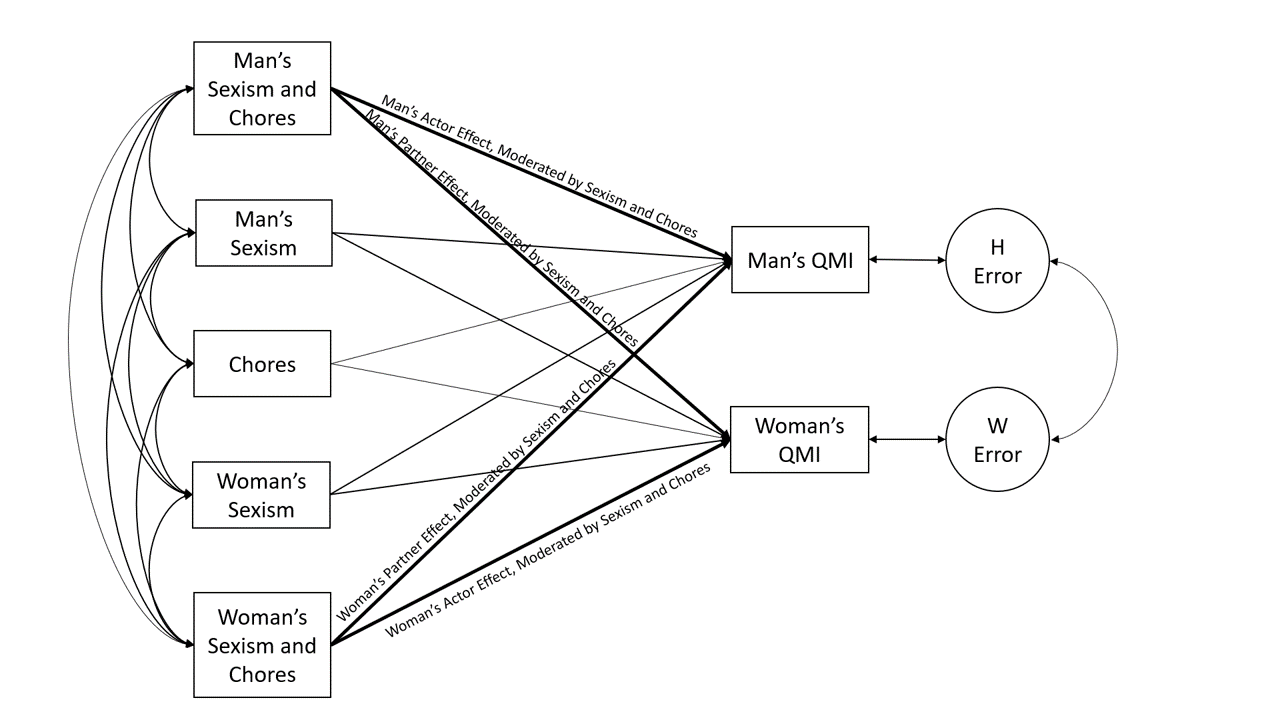
\includegraphics{APIM.png}
\caption{Our APIM Model}
\end{figure}

\emph{Note.}For simplicity, time was not included and HS and BS were simplified as sexism. In reality, HS and BS would interact with each other for both the actor and the partner.

\newpage

\hypertarget{references}{%
\section{References}\label{references}}

\begingroup
\setlength{\parindent}{-0.5in}
\setlength{\leftskip}{0.5in}

\hypertarget{refs}{}
\leavevmode\hypertarget{ref-R-papaja}{}%
Aust, F., \& Barth, M. (2020). \emph{papaja: Create APA manuscripts with R Markdown}. Retrieved from \url{https://github.com/crsh/papaja}

\leavevmode\hypertarget{ref-Bareket}{}%
Bareket, O., Shnabel, N., Kende, A., Knab, N., \& Bar-Anan, Y. (2020). Need some help, honey? Dependency-oriented helping relations between women and men in the domestic sphere. \emph{Journal of Personality and Social Psychology}, \emph{120}. \url{https://doi.org/10.1037/pspi0000292}

\leavevmode\hypertarget{ref-Barstad}{}%
Barstad, A. (2014). Equality is bliss? Relationship quality and the gender division of household labor. \emph{Journal of Family Issues}, \emph{35}(7), 972--992. \url{https://doi.org/10.1177/0192513X14522246}

\leavevmode\hypertarget{ref-R-Matrix}{}%
Bates, D., \& Maechler, M. (2021). \emph{Matrix: Sparse and dense matrix classes and methods}. Retrieved from \url{https://CRAN.R-project.org/package=Matrix}

\leavevmode\hypertarget{ref-Bick}{}%
Bick, B., Alexander, \& Mertens, K. (2020). Work from home after the covid-19 outbreak, (2017). \url{https://doi.org/10.24149/wp2017r2}

\leavevmode\hypertarget{ref-Braun}{}%
Braun, M., Lewin-Epstein, N., Stier, H., \& Baumgärtner, M. K. (2008). Perceived equity in the gendered division of household labor. \emph{Journal of Marriage and Family}, \emph{70}(5), 1145--1156. Retrieved from \url{http://www.jstor.org/stable/40056333}

\leavevmode\hypertarget{ref-Carlson}{}%
Carlson, M. W., \& Hans, J. D. (2020). Maximizing benefits and minimizing impacts: Dual-earner couples' perceived division of household labor decision-making process. \emph{Journal of Family Studies}, \emph{26}(2), 208--225. \url{https://doi.org/10.1080/13229400.2017.1367712}

\leavevmode\hypertarget{ref-Chen}{}%
Chen, Z., Fiske, S., \& Lee, T. (2009). Ambivalent sexism and power-related gender-role ideology in marriage. \emph{Sex Roles}, \emph{60}, 765--778. \url{https://doi.org/10.1007/s11199-009-9585-9}

\leavevmode\hypertarget{ref-Chesters}{}%
Chesters, J. (2013). Gender convergence in core housework hours: Assessing the relevance of earlier approaches for explaining current trends. \emph{Journal of Sociology}, \emph{49}, 78--96. \url{https://doi.org/10.1177/1440783311427482}

\leavevmode\hypertarget{ref-Doan}{}%
Doan, L., \& Quadlin, N. (2018). Partner characteristics and perceptions of responsibility for housework and child care. \emph{Journal of Marriage and Family}, \emph{81}. \url{https://doi.org/10.1111/jomf.12526}

\leavevmode\hypertarget{ref-Erickson}{}%
Erickson, R. (2005). Why emotion work matters: Sex, gender, and the division of household labor. \emph{Journal of Marriage and Family}, \emph{67}, 337--351. \url{https://doi.org/10.1111/j.0022-2445.2005.00120.x}

\leavevmode\hypertarget{ref-Glick1996}{}%
Glick, P., \& Fiske, S. (1996). The ambivalent sexism inventory: Differentiating hostile and benevolent sexism. \emph{Journal of Personality and Social Psychology}, \emph{70}, 491--512. \url{https://doi.org/10.1037/0022-3514.70.3.491}

\leavevmode\hypertarget{ref-ASI}{}%
Glick, P., \& Fiske, S. (1997). \emph{Psychology of Women Quarterly}, \emph{21}(1), 119--135. \url{https://doi.org/10.1111/j.1471-6402.1997.tb00104.x}

\leavevmode\hypertarget{ref-Glick2001}{}%
Glick, P., \& Fiske, S. (2001). An ambivalent alliance: Hostile and benevolent sexism as complementary justifications for gender inequality. \emph{The American Psychologist}, \emph{56}, 109--118. \url{https://doi.org/10.1037/0003-066X.56.2.109}

\leavevmode\hypertarget{ref-Greenstein2009}{}%
Greenstein, T. (2009). National context, family satisfaction, and fairness in the division of household labor. \emph{Journal of Marriage and Family}, \emph{71}, 1039--1051. \url{https://doi.org/10.1111/j.1741-3737.2009.00651.x}

\leavevmode\hypertarget{ref-Greenstein1996}{}%
Greenstein, T. N. (1996). Husbands' participation in domestic labor: Interactive effects of wives' and husbands' gender ideologies. \emph{Journal of Marriage and Family}, \emph{58}(3), 585--595. Retrieved from \url{http://www.jstor.org/stable/353719}

\leavevmode\hypertarget{ref-R-lubridate}{}%
Grolemund, G., \& Wickham, H. (2011). Dates and times made easy with lubridate. \emph{Journal of Statistical Software}, \emph{40}(3), 1--25. Retrieved from \url{https://www.jstatsoft.org/v40/i03/}

\leavevmode\hypertarget{ref-Hammond}{}%
Hammond, M. D., \& Overall, N. C. (2013). When relationships do not live up to benevolent ideals: Women's benevolent sexism and sensitivity to relationship problems. \emph{European Journal of Social Psychology}, \emph{43}(3), 212--223. \url{https://doi.org/https://doi.org/10.1002/ejsp.1939}

\leavevmode\hypertarget{ref-Helms}{}%
Helms, H. M., Walls, J. K., Crouter, A. C., \& McHale, S. M. (2010). Provider role attitudes, marital satisfaction, role overload, and housework: A dyadic approach. \emph{Journal of Family Psychology : JFP : Journal of the Division of Family Psychology of the American Psychological Association}, \emph{24 5}, 568--577.

\leavevmode\hypertarget{ref-R-purrr}{}%
Henry, L., \& Wickham, H. (2020). \emph{Purrr: Functional programming tools}. Retrieved from \url{https://CRAN.R-project.org/package=purrr}

\leavevmode\hypertarget{ref-R-ggstance}{}%
Henry, L., Wickham, H., \& Chang, W. (2020). \emph{Ggstance: Horizontal 'ggplot2' components}. Retrieved from \url{https://CRAN.R-project.org/package=ggstance}

\leavevmode\hypertarget{ref-Huffman}{}%
Huffman, A., Matthews, R., \& Irving, L. (2016). Family fairness and cohesion in marital dyads: Mediating processes between work--family conflict and couple psychological distress. \emph{Journal of Occupational and Organizational Psychology}, \emph{90}. \url{https://doi.org/10.1111/joop.12165}

\leavevmode\hypertarget{ref-R-ggformula}{}%
Kaplan, D., \& Pruim, R. (2021). \emph{Ggformula: Formula interface to the grammar of graphics}. Retrieved from \url{https://CRAN.R-project.org/package=ggformula}

\leavevmode\hypertarget{ref-Kenny}{}%
Kenny, D., Kashy, D., Cook, W., \& Simpson, J. (2006). \emph{Dyadic data analysis}. \emph{American Statistician - AMER STATIST} (Vol. 61).

\leavevmode\hypertarget{ref-Lam}{}%
Lam, C. B., McHale, S. M., \& Crouter, A. C. (2012). The division of household labor: Longitudinal changes and within-couple variation. \emph{Journal of Marriage and Family}, \emph{74}(5), 944--952. \url{https://doi.org/https://doi.org/10.1111/j.1741-3737.2012.01007.x}

\leavevmode\hypertarget{ref-Lee}{}%
Lee, T., Fiske, S., Glick, P., \& Chen, Z. (2010). Ambivalent sexism in close relationships: (Hostile) power and (benevolent) romance shape relationship ideals. \emph{Sex Roles}, \emph{62}, 583--601. \url{https://doi.org/10.1007/s11199-010-9770-x}

\leavevmode\hypertarget{ref-Minnotte}{}%
Minnotte, K., Minnotte, M., \& Pedersen, D. (2013). Marital satisfaction among dual‐Earner couples: Gender ideologies and family‐to‐Work conflict. \emph{Family Relations}, \emph{62}. \url{https://doi.org/10.1111/fare.12021}

\leavevmode\hypertarget{ref-R-tibble}{}%
Müller, K., \& Wickham, H. (2021). \emph{Tibble: Simple data frames}. Retrieved from \url{https://CRAN.R-project.org/package=tibble}

\leavevmode\hypertarget{ref-Nordenmark}{}%
Nordenmark, M., \& Nyman, C. (2003). Fair or unfair? Perceived fairness of household division of labour and gender equality among women and men the swedish case. \emph{European Journal of Women's Studies}, \emph{10}, 181--209. \url{https://doi.org/10.1177/1350506803010002004}

\leavevmode\hypertarget{ref-R-nlme}{}%
Pinheiro, J., Bates, D., DebRoy, S., Sarkar, D., \& R Core Team. (2022). \emph{nlme: Linear and nonlinear mixed effects models}. Retrieved from \url{https://CRAN.R-project.org/package=nlme}

\leavevmode\hypertarget{ref-Poortman}{}%
Poortman, A.-R., \& Lippe, T. V. D. (2009). Attitudes toward housework and child care and the gendered division of labor. \emph{Journal of Marriage and Family}, \emph{71}(3), 526--541. Retrieved from \url{http://www.jstor.org/stable/40262900}

\leavevmode\hypertarget{ref-R-mosaicData}{}%
Pruim, R., Kaplan, D., \& Horton, N. (2021). \emph{MosaicData: Project mosaic data sets}. Retrieved from \url{https://CRAN.R-project.org/package=mosaicData}

\leavevmode\hypertarget{ref-R-mosaic}{}%
Pruim, R., Kaplan, D. T., \& Horton, N. J. (2017). The mosaic package: Helping students to 'think with data' using r. \emph{The R Journal}, \emph{9}(1), 77--102. Retrieved from \url{https://journal.r-project.org/archive/2017/RJ-2017-024/index.html}

\leavevmode\hypertarget{ref-R-base}{}%
R Core Team. (2022). \emph{R: A language and environment for statistical computing}. Vienna, Austria: R Foundation for Statistical Computing. Retrieved from \url{https://www.R-project.org/}

\leavevmode\hypertarget{ref-R-psych}{}%
Revelle, W. (2021). \emph{Psych: Procedures for psychological, psychometric, and personality research}. Evanston, Illinois: Northwestern University. Retrieved from \url{https://CRAN.R-project.org/package=psych}

\leavevmode\hypertarget{ref-R-lattice}{}%
Sarkar, D. (2008). \emph{Lattice: Multivariate data visualization with r}. New York: Springer. Retrieved from \url{http://lmdvr.r-forge.r-project.org}

\leavevmode\hypertarget{ref-Thomae}{}%
Thomae, M., \& Houston, D. (2016). The impact of gender ideologies on men's and women's desire for a traditional or non-traditional partner. \emph{Personality and Individual Differences}, \emph{95}, 152--158. \url{https://doi.org/10.1016/j.paid.2016.02.026}

\leavevmode\hypertarget{ref-R-ggplot2}{}%
Wickham, H. (2016). \emph{Ggplot2: Elegant graphics for data analysis}. Springer-Verlag New York. Retrieved from \url{https://ggplot2.tidyverse.org}

\leavevmode\hypertarget{ref-R-stringr}{}%
Wickham, H. (2019). \emph{Stringr: Simple, consistent wrappers for common string operations}. Retrieved from \url{https://CRAN.R-project.org/package=stringr}

\leavevmode\hypertarget{ref-R-forcats}{}%
Wickham, H. (2021). \emph{Forcats: Tools for working with categorical variables (factors)}. Retrieved from \url{https://CRAN.R-project.org/package=forcats}

\leavevmode\hypertarget{ref-R-tidyverse}{}%
Wickham, H., Averick, M., Bryan, J., Chang, W., McGowan, L. D., François, R., \ldots{} Yutani, H. (2019). Welcome to the tidyverse. \emph{Journal of Open Source Software}, \emph{4}(43), 1686. \url{https://doi.org/10.21105/joss.01686}

\leavevmode\hypertarget{ref-R-dplyr}{}%
Wickham, H., François, R., Henry, L., \& Müller, K. (2022a). \emph{Dplyr: A grammar of data manipulation}. Retrieved from \url{https://CRAN.R-project.org/package=dplyr}

\leavevmode\hypertarget{ref-R-tidyr}{}%
Wickham, H., \& Girlich, M. (2022). \emph{Tidyr: Tidy messy data}. Retrieved from \url{https://CRAN.R-project.org/package=tidyr}

\leavevmode\hypertarget{ref-R-readr}{}%
Wickham, H., Hester, J., \& Bryan, J. (2022b). \emph{Readr: Read rectangular text data}. Retrieved from \url{https://CRAN.R-project.org/package=readr}

\leavevmode\hypertarget{ref-R-gtable}{}%
Wickham, H., \& Pedersen, T. L. (2019). \emph{Gtable: Arrange 'grobs' in tables}. Retrieved from \url{https://CRAN.R-project.org/package=gtable}

\leavevmode\hypertarget{ref-R-ggridges}{}%
Wilke, C. O. (2021). \emph{Ggridges: Ridgeline plots in 'ggplot2'}. Retrieved from \url{https://CRAN.R-project.org/package=ggridges}

\leavevmode\hypertarget{ref-R-kableExtra}{}%
Zhu, H. (2021). \emph{KableExtra: Construct complex table with 'kable' and pipe syntax}. Retrieved from \url{https://CRAN.R-project.org/package=kableExtra}

\endgroup


\end{document}
